\section{Basic design}


\subsection{Data structure}

The local state of a node in the StreamNet protocol is a direct acyclic graph (DAG) $G = <B,g,P,E>$. 
$B$ is the set of blocks in $G$. 
$g \in G$ is the genesis block. 
For instance, vertex $g$ in Figure~\ref{simple_sn} represents the Genesis block.
$P$ is a function that maps a block $b$ to its parent block $P(b)$. Specially, $P(g) = \perp$. 
In Figure~\ref{simple_sn}, parent relationships are denoted by solid edges.
Note that there is always a parent edge from a block to its parent block (i.e., $\forall b \in B$, $b, P(b)> \in E$). 
$E$ is the set of directly reference edges and parent edges in this graph. 
$e = <b,b'> \in E$ is an edge from the block $b$ to the block $b'$, 
which means that $b'$ happens before $b$. 
For example in Figure~\ref{simple_sn}, vertex $1$ represents the first block, which is referenced by the subsequent block $2$, $3$ and $4$. 
Vertex $5$ has two edges, one is the parent edge pointing to $3$, another is reference edge pointing to $4$.
When a new block is not referenced, it is called a tip. For example, in Figure~\ref{simple_sn}, block $6$ is a tip.
All blocks in the StreamNet protocol share a predefined deterministic 
hash function Hash that maps each block in $B$ to a unique integer id . 
It satisfies that $\forall {b} \neq {b'}$, Hash($b$) $\neq$ Hash($b'$).

\begin{figure}[!ht]
\begin{center}
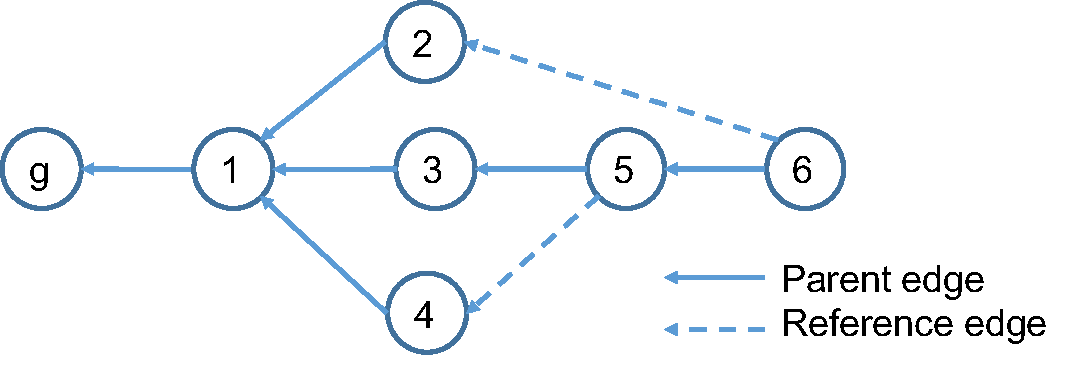
\includegraphics[width=0.45\textwidth]{figures/simple_sn.pdf}
    \caption{
        Example of the StreamNet data structure.
     }
\label{simple_sn}
\end{center}
\end{figure}

\subsection{StreamNet Architecture}

Figure~\ref{architecture} presents the architecture of StreamNet,
it's consists of multiple StreamNet machines.
Each StreamNet machine will grow its DAG locally, and will broadcast the changes using gossip protocol. 
Eventually, every machine will have a unified view of DAG.
By calling total ordering algorithm, every machine can sort the DAG into a total order, 
and the data in each block can have a relative order regardless of their local upload time.
Figure~\ref{node} shows the local architecture of StreamNet.
In each StreamNet node, there will be a transaction pool accecpting the transactions from the HTTP API.
And there will be a block generator to pack a certain amount of transactions into a block, it firstly find a 
parent and reference block to attach the new block to, based on the hash information of these two blocks and the meta data of the block itself, 
it will then perform the proof of work (POW) to calculate the nonce for the received block.
Agorithm~\ref{algo:main_loop} summarize the server logic for a StreamNet node.
In the algorithm, the way to find parent reference node is by $Pivot(G, g)$.
And the way to find reference node is by calling $MCMC(G, g)$ which is the Markov Chain Monte Carlo (MCMC) random walk algorithm \cite{popov2016tangle}.
The two algorithms will be described in the later section.

\begin{figure}[!ht]
\begin{center}
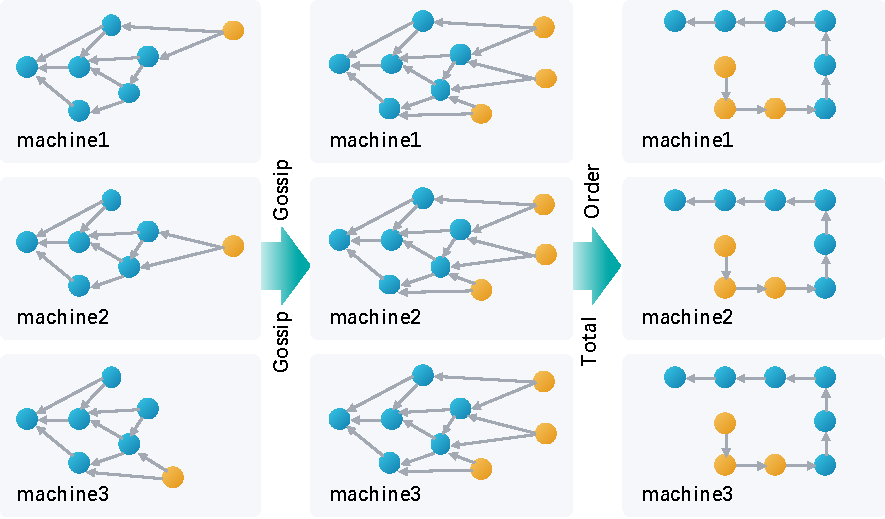
\includegraphics[width=0.45\textwidth]{figures/architecture.pdf}
    \caption{
        StreamNet architecture.
     }
\label{architecture}
\end{center}
\end{figure}

\begin{figure}[!ht]
\begin{center}
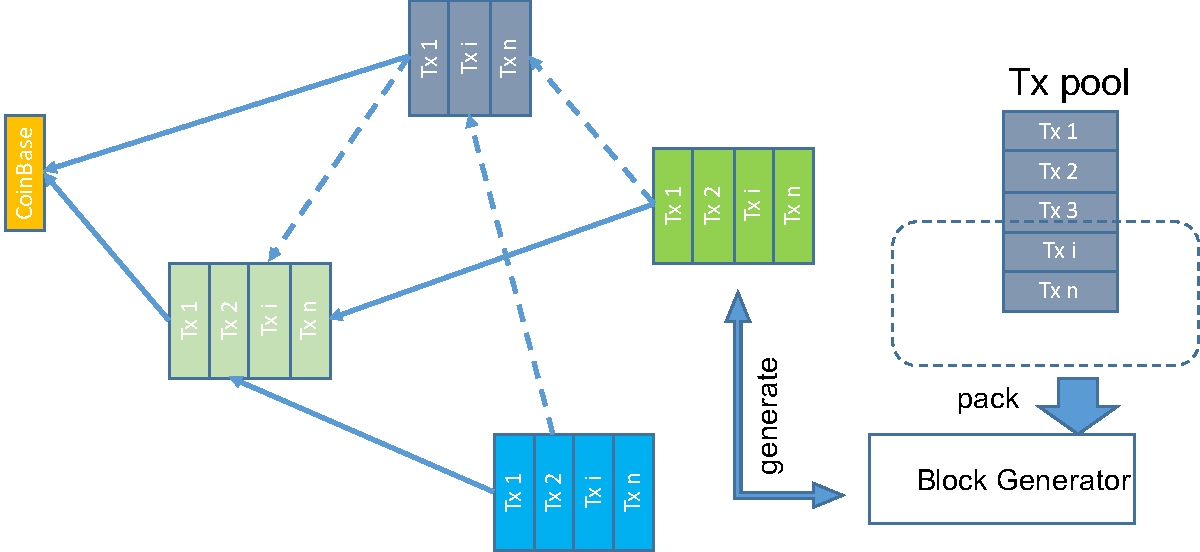
\includegraphics[width=0.45\textwidth]{figures/node.pdf}
    \caption{
        One node in StreamNet protocol.
     }
\label{node}
\end{center}
\end{figure}

\IncMargin{1em}
\begin{algorithm}
\SetKwData{Left}{left}\SetKwData{This}{this}\SetKwData{Up}{up}
\SetKwFunction{Union}{Union}\SetKwFunction{FindCompress}{FindCompress}
\SetKwInOut{Input}{input}\SetKwInOut{Output}{output}

\KwIn{ Graph $G=<B, g, P, E>$ }

    \While {Node is running}{
        \uIf{Received $G' = <B', g, P', E'> $}{
            $G'' \gets <B \cup B', g, P \cup P', E \cup E' > $\;
            \uIf{$G \neq G''$ } {
                $G \gets G''$ \;
                Broadcase updated G to neighbors \;
            }
        } 

        \uIf{Generate block $b$}{
            $a \gets Pivot(G, g) $ \;
            $r \gets MCMC(G, g) $ \;
            $G \gets <B \cup b, g, P \cup <b, a>, E \cup <b, a> \cup <b, r> >$ \;
            Broadcase updated G to neighbors \;
        } 
    }

\caption{{ StreamNet node main loop.}}
\label{algo:main_loop}
\end{algorithm}
\DecMargin{1em}


\IncMargin{1em}
\begin{algorithm}
\SetKwData{Left}{left}\SetKwData{This}{this}\SetKwData{Up}{up}
\SetKwFunction{Union}{Union}\SetKwFunction{FindCompress}{FindCompress}
\SetKwInOut{Input}{input}\SetKwInOut{Output}{output}

\KwIn{ The local state $G$ = $<B,g,P,E>$  and a starting block $b \in B$ }
\KwOut{ A random tip $t$ }

$t \leftarrow b$

\Do { Score(G,t) != 0} {
    \For {$b' \in Child(G,t)$} {
        $P_{bb'} = \frac{e^{\alpha Score(G,b')}}{\Sigma_{z:z \rightarrow b}e^{\alpha Score(G,z)}}$
    }
    $t \leftarrow $ choose $b''$ by $P_{bb''}$
}

\Return{$t$} \;

\caption{{\sc MCMC($G$, $b$).}}
\label{algo:mcmc}
\end{algorithm}
\DecMargin{1em}



\subsection{Consensus protocol}
Based on predefineid data structure, to present the StreamNet consensus algorithm, 
we firstly define several utility functions and notatons, which is a variation from the definition in the Conflux paper \cite{li2018scaling}. 
Chain() returns the chain from the genesis block to a given block following only parent edges. 
Child() returns the set of child blocks of a given block. 
Sibling() returns the set of siblings of a given block. 
Subtree() returns the sub-tree of a given block in the parental tree. 
Before() returns the set of blocks that are immediately generated before a given block. 
Past() returns the set of blocks that are generated before a given block (but including the block itself).
After() returns the set of blocks that are immediately generated after a given block. 
Later() returns the set of blocks that are generated after a given block (but including the block itself).
SubGraph() returns the sub graph by removing blocks and edges except the initial set of blocks.
ParentScore() presents the weight of blocks, each block have a score when referenced as parent. 
Score() presents the weight of blocks, each block achieves a score when attaching to the graph. 
TotalOrder() returns the `flattend' order infered from the consensus algorithm.
Figure~\ref{allMethods} represents the definition of these utility functions. 

\begin{figure}
\begin{flalign*}
  &\fbox{G = $<B,g,P,E>$} \\
  &Chain(G,b) =
  \begin{cases}
    g                 & \text{b = g} \\
    Chain(G,P(b))     & \text{otherwise}
  \end{cases} \\
   &Child(G,b) = \{ b'| P(b') = b \} \\
   &Sibling(G,b) = Child(G,P(b)) \\
   &SubTree(G,b) = (U_{i\in Child(G,b)}Substree(G,i))U\{b\} \\
   &Before(G,b) = \{b'|b' \in B, <b,b'> \in E \} \\
   &Past(G,b) = (U_{i\in Before(G,b)}Past(G,i))U\{b\} \\
   &After(G,b) = \{b'|b' \in B, <b',b> \in E \} \\
   &Later(G,b) = (U_{i\in After(G,b)}Later(G,i))U\{b\} \\
   &SubGraph(G,B') = <B', P', E'> | \\
   & \forall <b, b'> \in E', b \subset B' \& b' \subset B'\\
   &ParentScore(G,b) = |SubTree(G,b)| \\
   &Score(G,b) = |Later(G,b)| \\
   &TotalOrder(G) = StreamNetOrder(G,Pivot(G,g)) 
\end{flalign*}

    \caption{The Definitions of Chain(), Child(), Sibling(), Subtree(), Before(), Past(), After(), Later(), SubGraph(), ParentScore(), Score(), and TotalOrder(). }
\label{allMethods}
\end{figure}


\subsubsection{Parent tip Selection by pivotal chain} 
The algorithm Algorithm~\ref{algo:getPivot} presents our pivot chain selection algorithm(i.e., the definition of $Pivot(G, b)$). 
Given a StreamNet state $G$, Pivot($G$,$g$) returns the last block in the pivot chain starting from the genesis block $g$. 
The algorithm recursively advances to the child block whoes corresponding subtree has the largest number of blocks. 
Which is calculated by $Score(G, b)$  
When there are multiple child blocks with the same score, the algorithm selects the child block with the largest block hash. 
The algorithm terminates until it reaches a tip. 
Each block in the pivot chain defines a epoch in the DAG, the nodes in DAG that satisfy Past($G$,$b$) - Past($G$,$p$) will belong to the epoch of block $b$.
For example, in Figure~\ref{total_order}, the pivot chain is $<g, 1, 3, 5, 6>$, and the epoch of block $5$ contains two blocks $4$ and $5$.

\IncMargin{1em}
\begin{algorithm}
\SetKwData{Left}{left}\SetKwData{This}{this}\SetKwData{Up}{up}
\SetKwFunction{Union}{Union}\SetKwFunction{FindCompress}{FindCompress}
\SetKwInOut{Input}{input}\SetKwInOut{Output}{output}

\KwIn{ The local state $G$ = $<B,g,P,E>$  and a starting block $b \in B$ }
\KwOut{ The last block in the pivot chain for the subtree of $b$ in $G$ }

\Do { Child(G,b) != 0} {
  $b'$ $\longleftarrow$ Child($G,b$)  \;
  $tmpMaxScore$ $\longleftarrow$ -1 \;
  $tmpBlock$ $\longleftarrow$ $\perp$ \;
  \Do { $b'$ $\neq$ 0 } {
    $score$ $\longleftarrow$ Score($G, b'$) \;
    \If { $score$ $>$ $tmpMaxScore$ $||$ ($score$ = $tmpMaxScore$ and \text{the score of $b'$ gather than $tmpBlock$})} {
      $tmpMaxScore$ $\longleftarrow$ $score$ \;
      $tmpBlock$ $\longleftarrow$ $b'$ \; 
    }
  }
  $b$ $\longleftarrow$ $tmpBlock$ \;
}

\Return{$tmpBlock$} \;

\caption{{\sc pivot block($G$, $b$).}}
\label{algo:getPivot}
\end{algorithm}
\DecMargin{1em}



\subsubsection{Reference tip selection by MCMC} 

The tip selection method by using Monte Carlo Random Walk (MCMC) is as Algorithm~\ref{algo:mcmc} shows.
Starting from the genesis, each random walk step will choose a child to jump to,
and the probability of jumping from one block to the next block will be calculated using the formula in the algorithm.
$\alpha$ in the formula is an constant that is used to scale the randomness of the MCMC function, the smaller it is, the more randomness will be in the MCMC function.
The algorithnm returns until it finds a tip.

\subsubsection{Total Order} 
The algorithm Algorithm~\ref{algo:conflux_order} defines StreamNetOrder(), 
which corresponds to our block ordering algorithm. 
Given the local state $G$ and a block $a$ in the pivot chain, 
StreamNetOrder($G$,$a$) returns the ordered list of all blocks that appear in or before the epoch of $a$. 
Using StreamNetOrder(), the total order of a local state $G$ is defined as TotalOrder($G$) in Figure~\ref{total_order}. 
The algorithm in Figure~\ref{total_order}  first recursively orders all blocks in previous epochs(i.e., the epoch of $P(a)$ and before). 
It then computes all blocks in the epoch of $a$ as $B_\Delta$. 
It topologically sorts all blocks in $B_\Delta$ and appends it into the result list. 
The algorithm uses the unique hash to break ties. 

\IncMargin{1em}
\begin{algorithm}
\SetKwData{Left}{left}\SetKwData{This}{this}\SetKwData{Up}{up}
\SetKwFunction{Union}{Union}\SetKwFunction{FindCompress}{FindCompress}
\SetKwInOut{Input}{input}\SetKwInOut{Output}{output}

\KwIn{ The local state $G$ = $<B,g,P,E>$  and a tip block $b \in B$ }
\KwOut{ The block list of total top order starting from Genesis block to the giving block $b$ in $G$ }

$L = \perp$

\Do { $b$ != $g$} {
  $p$ $\gets$ Parent($G,b$)  \;
  $B_\Delta$ $\gets$ Past($G$,$b$) - Past($G$,$p$) \;
  \Do { $B_\Delta$ $\neq$ 0 } {
      $G'$ $\gets SubGraph(B_\Delta) $ \;
    $B'_\Delta$ $\gets$ \{x $||$ Before($G'$,$x$) = 0\} \;
    \text{Sort all blocks in $B'_\Delta$ in order as $b'_1,b'_2,...,b'_k$} \\
      \text{such that $\forall$1$\leq i \leq j \leq k$, Hash($b'_i$) $\leq$ Hash($b'_j$)} \;  
    $L$ $\gets$ $L + b'_1 + b'_2 + ... + b'_k$ \;
    $B_\Delta$ $\gets$ $B_\Delta$ - $B'_\Delta$ \;
  }
  $b$ = $p$ \;
}


\Return{$L$} \;

\caption{{\sc StreamNetOrder($G$, $b$).}}
\label{algo:conflux_order}
\end{algorithm}
\DecMargin{1em}


\begin{figure}[!ht]
\begin{center}
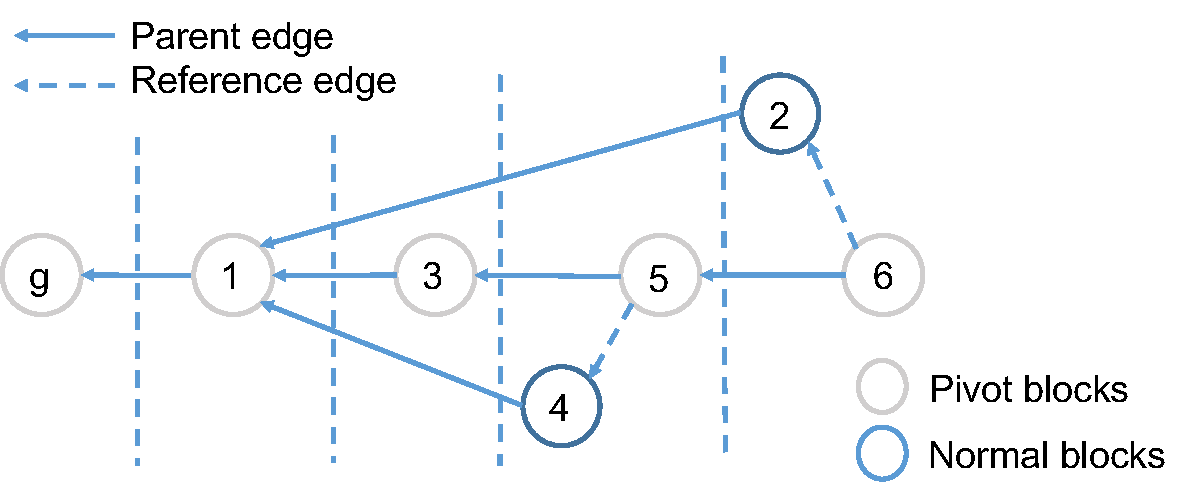
\includegraphics[width=0.45\textwidth]{figures/total_order.pdf}
    \caption{
        An example of total order calculation.
     }
\label{total_order}
\end{center}
\end{figure}

\subsection{The UTXO model}

In StreamNet, the transactions utilizes the unspent transaction out (UTXO) model, which is exactly the same as in Bitcoin.
In the confirmation process, the user will call $TotalOrder$ to get the relative order of different blocks, 
and the conflict content of the block will be eliminated if the order of the block is later than the one conflicting with it in the total order.
Figure ~\ref{utxo} shows the example of storage of UTXO in StreamNet and how conifliction is resolved.
Two blocks both referenced the same block with Alice having 5 tokens, and construct the new transaction out which representing the transfer of token to Bob and Jack respectively.
However, after calling $totalOrder()$, the Bob transfer block preceeds the Jack transfer block, thus the later block will be discarded.

\begin{figure}[!ht]
\begin{center}
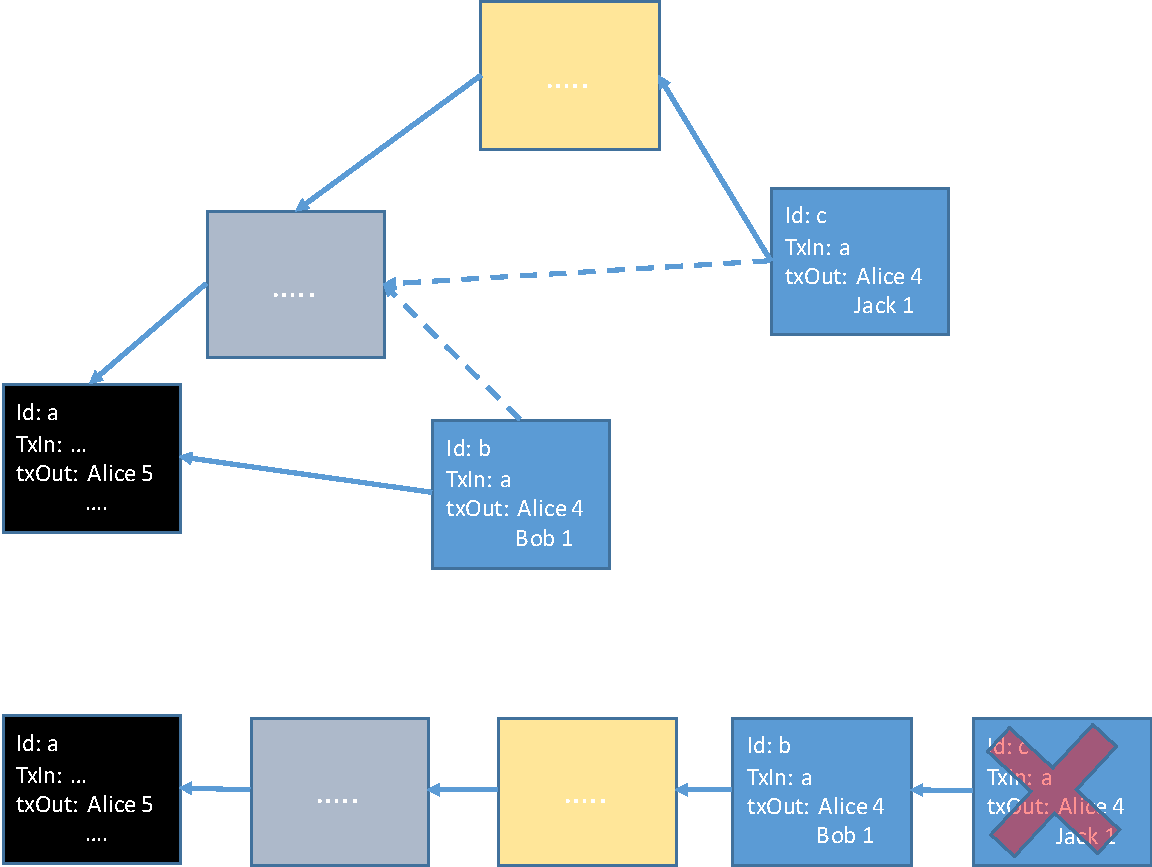
\includegraphics[width=0.45\textwidth]{figures/utxo.pdf}
    \caption{
        An example of UTXO.
     }
\label{utxo}
\end{center}
\end{figure}

\subsection{Gossip Network}
In the bitcoin and IOTA network, the block information is diseminated in a direct mail way \cite{demers1988epidemic}.
Suppose there are $N$ nodes and $L$ links in the network, for a block of size $B$,
to spread the information of it, the direct mail algorithm will have a total complexity of $O(LB)$.
And the average complexity for a node will be $O(\frac{LB}{N})$
In the chain based system, this is fine, because the design of the system already assume that the transaction rate will be low.
However, in the DAG based system, this type of gossip manner will result in low scalability due to the network flooding.
What's worse, consider the heterogenerously and long diameters of network topology, the convergence of DAG will take long time which will result in the delay of confirmation time of blocks.

There are solutions in \cite{demers1988epidemic}, and in Hyperledger \cite{androulaki2018hyperledger} 
they have adopted the PUSH and PULL model for the gossip message propogation. However, their system is aiming at small scale. 
Suppose the size of the hash of a block is $H$, we designed the direct signal algorithm. 
The algorithm is divided into two steps, once a node generate or receive a block, 
it firstly broadcast the hash of the block, this is the PUSH step. 
Once a node receive a hash or a set of a hash,
it will pick one source of the hash for the block content, this is the PULL step.
The direct signal algorithm's complexity will be $O(LH + NB)$ and for a node averaged to $O(\frac{LH}{N} + 1)$
The algorithm is as Algorithm~\ref{algo:gossip} shows.

\IncMargin{1em}
\begin{algorithm}
\SetKwData{Left}{left}\SetKwData{This}{this}\SetKwData{Up}{up}
\SetKwFunction{Union}{Union}\SetKwFunction{FindCompress}{FindCompress}
\SetKwInOut{Input}{input}\SetKwInOut{Output}{output}

\KwIn{ Graph $G=<B, g, P, E>$ }

    \While {Node is running}{
        \uIf{Received or Generate block $b$}{
            $h \gets Hash(b)$ \;
            $cache[h] \gets b$ \;
            Broadcast $h$ to neighbors \;
        } 

        \uIf{Received request of $h$ from neighbor $n$ }{
            $b \gets cache[h]$ \;
            Send $b$ to $n$ \;
        } 

        \uIf{Received hash $h$ from neighbor $n$}{
            $b \gets cache[h]$ \;
            \uIf{ $b = NULL $ } {  
                Send request $h$ to $n$ \;
            }
        } 
    }

\caption{{ Gossip Algorithm.}}
\label{algo:gossip}
\end{algorithm}
\DecMargin{1em}


\subsection{Differences with other DAG protocols}
Here, we mainly compare the difference of our protocol with two mainstream DAG based protocols, one is IOTA, another is Conflux.

\subsubsection{IOTA}
The major difference with IOTA are in three points:
\begin{itemize}
    \item Firstly, the IOTA tip selection algorithm's two tips are all randomly choosen, 
        and ours is one deterministic which is for the total ordering purposes and one by random which is for maintaining the DAG property; 
    \item Secondly, the IOTA consensus algorithm is not purely decentralized, 
        it relies on a central coordinator to issue milestones for multiple purposes, and our algorithm does not dependent on such facility. 
    \item Lastly, in IOTA, there is no concept of total order,
        and there are 3 ways to judge if a transaction is confirmed: 
    \begin{itemize}
        \item The first way is that the common nodes covered by all the tips are considered to be fully confirmed; 
        \item All transactions referenced by the milestone tip are confirmed.
        \item The third way is to use MCMC.
            Call $N$ times to select a tip using the tip selection algorithm.
            If a block is referenced by this tip, its credibility is increased by 1.
            After $N$ selections have been cited $M$ times, then the credibility is $M / N$.
    \end{itemize}
\end{itemize}

\subsubsection{Conflux}
The major difference with Conflux are in two points:
\begin{itemize}
    \item Firstly, Conflux will approve all tips in the DAG along with parent, which is much more complicated than our MCMC based two tip method. 
        And when the width of DAG is high, there will be much more space needed to maintain such data structure. 
    \item Secondly, Conflux total ordering algorithm advances from genesis block to the end while StreamNet advances in the reverse direction. 
        This method is one of the major contribution to our streaming graph based optimizations,
        which will be discussed in the next chapter. 
        In Conflux paper, there is no description of how to deal with the complexity paired with the growing graph.
\end{itemize}
